121. В $1\text{см}^2$ содержится $2\cdot2=4$ клетки, значит необходимо нарисовать десятиугольник, состоящий из $4\cdot10+4:2=42$ клеток. Один из возможных примеров изображён ниже.
\begin{center}
\begin{figure}[ht!]
\center{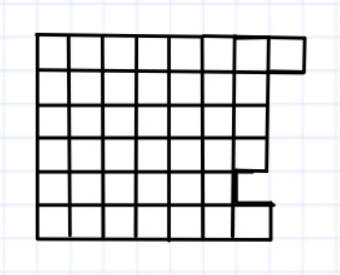
\includegraphics[scale=0.35]{2222.png}}
\end{figure}
\end{center}
